\documentclass[twoside]{book}

% Packages required by doxygen
\usepackage{fixltx2e}
\usepackage{calc}
\usepackage{doxygen}
\usepackage[export]{adjustbox} % also loads graphicx
\usepackage{graphicx}
\usepackage[utf8]{inputenc}
\usepackage{makeidx}
\usepackage{multicol}
\usepackage{multirow}
\PassOptionsToPackage{warn}{textcomp}
\usepackage{textcomp}
\usepackage[nointegrals]{wasysym}
\usepackage[table]{xcolor}

% NLS support packages
\usepackage[french]{babel}

% Font selection
\usepackage[T1]{fontenc}
\usepackage[scaled=.90]{helvet}
\usepackage{courier}
\usepackage{amssymb}
\usepackage{sectsty}
\renewcommand{\familydefault}{\sfdefault}
\allsectionsfont{%
  \fontseries{bc}\selectfont%
  \color{darkgray}%
}
\renewcommand{\DoxyLabelFont}{%
  \fontseries{bc}\selectfont%
  \color{darkgray}%
}
\newcommand{\+}{\discretionary{\mbox{\scriptsize$\hookleftarrow$}}{}{}}

% Page & text layout
\usepackage{geometry}
\geometry{%
  a4paper,%
  top=2.5cm,%
  bottom=2.5cm,%
  left=2.5cm,%
  right=2.5cm%
}
\tolerance=750
\hfuzz=15pt
\hbadness=750
\setlength{\emergencystretch}{15pt}
\setlength{\parindent}{0cm}
\setlength{\parskip}{0.2cm}
\makeatletter
\renewcommand{\paragraph}{%
  \@startsection{paragraph}{4}{0ex}{-1.0ex}{1.0ex}{%
    \normalfont\normalsize\bfseries\SS@parafont%
  }%
}
\renewcommand{\subparagraph}{%
  \@startsection{subparagraph}{5}{0ex}{-1.0ex}{1.0ex}{%
    \normalfont\normalsize\bfseries\SS@subparafont%
  }%
}
\makeatother

% Headers & footers
\usepackage{fancyhdr}
\pagestyle{fancyplain}
\fancyhead[LE]{\fancyplain{}{\bfseries\thepage}}
\fancyhead[CE]{\fancyplain{}{}}
\fancyhead[RE]{\fancyplain{}{\bfseries\leftmark}}
\fancyhead[LO]{\fancyplain{}{\bfseries\rightmark}}
\fancyhead[CO]{\fancyplain{}{}}
\fancyhead[RO]{\fancyplain{}{\bfseries\thepage}}
\fancyfoot[LE]{\fancyplain{}{}}
\fancyfoot[CE]{\fancyplain{}{}}
\fancyfoot[RE]{\fancyplain{}{\bfseries\scriptsize Généré le Jeudi 10 Décembre 2015 18\+:32\+:56 pour Exemple 0 par Doxygen }}
\fancyfoot[LO]{\fancyplain{}{\bfseries\scriptsize Généré le Jeudi 10 Décembre 2015 18\+:32\+:56 pour Exemple 0 par Doxygen }}
\fancyfoot[CO]{\fancyplain{}{}}
\fancyfoot[RO]{\fancyplain{}{}}
\renewcommand{\footrulewidth}{0.4pt}
\renewcommand{\chaptermark}[1]{%
  \markboth{#1}{}%
}
\renewcommand{\sectionmark}[1]{%
  \markright{\thesection\ #1}%
}

% Indices & bibliography
\usepackage{natbib}
\usepackage[titles]{tocloft}
\setcounter{tocdepth}{3}
\setcounter{secnumdepth}{5}
\makeindex

% Custom commands
\newcommand{\clearemptydoublepage}{%
  \newpage{\pagestyle{empty}\cleardoublepage}%
}


%===== C O N T E N T S =====

\begin{document}

% Titlepage & ToC
\pagenumbering{roman}
\begin{titlepage}
\vspace*{7cm}
\begin{center}%
{\Large Exemple 0 \\[1ex]\large 0.\+1 }\\
\vspace*{1cm}
{\large Généré par Doxygen 1.8.10}\\
\vspace*{0.5cm}
{\small Jeudi 10 Décembre 2015 18:32:56}\\
\end{center}
\end{titlepage}
\clearemptydoublepage
\tableofcontents
\clearemptydoublepage
\pagenumbering{arabic}

%--- Begin generated contents ---
\chapter{Index hiérarchique}
\section{Hiérarchie des classes}
Cette liste d\textquotesingle{}héritage est classée approximativement par ordre alphabétique \+:\begin{DoxyCompactList}
\item \contentsline{section}{Classe\+A}{\pageref{class_classe_a}}{}
\begin{DoxyCompactList}
\item \contentsline{section}{Classe\+De\+Base}{\pageref{class_classe_de_base}}{}
\end{DoxyCompactList}
\item \contentsline{section}{Classe\+B}{\pageref{class_classe_b}}{}
\item \contentsline{section}{Classe\+C}{\pageref{class_classe_c}}{}
\begin{DoxyCompactList}
\item \contentsline{section}{Classe\+De\+Base}{\pageref{class_classe_de_base}}{}
\end{DoxyCompactList}
\end{DoxyCompactList}

\chapter{Index des classes}
\section{Liste des classes}
Liste des classes, structures, unions et interfaces avec une brève description \+:\begin{DoxyCompactList}
\item\contentsline{section}{{\bf Classe\+A} \\*Dans la \doxyref{Classe\+A}{p.}{class_classe_a} on colle une définition de type et on utilise ce type dans 2 attributs associés en multiple (dans des vectors ($\ast$) }{\pageref{class_classe_a}}{}
\item\contentsline{section}{{\bf Classe\+B} \\*Associé avec le type\+: \textquotesingle{}Aggregation\textquotesingle{}. Créer l\textquotesingle{}attribut dans un shared\+\_\+ptr }{\pageref{class_classe_b}}{}
\item\contentsline{section}{{\bf Classe\+C} \\*Ici on associe 2 stereotypes \+: un using et un enum }{\pageref{class_classe_c}}{}
\item\contentsline{section}{{\bf Classe\+De\+Base} \\*Classe qui hérite de 2 autres classes. Cela ajoutera les includes necéssaires }{\pageref{class_classe_de_base}}{}
\end{DoxyCompactList}

\chapter{Index des fichiers}
\section{Liste des fichiers}
Liste de tous les fichiers avec une brève description \+:\begin{DoxyCompactList}
\item\contentsline{section}{R\+:/06 -\/ C++/dia2code\+Perso/exemple/code\+C\+P\+P\+\_\+exemple 0/include/{\bf Classe\+A.\+h} }{\pageref{_classe_a_8h}}{}
\item\contentsline{section}{R\+:/06 -\/ C++/dia2code\+Perso/exemple/code\+C\+P\+P\+\_\+exemple 0/include/{\bf Classe\+B.\+h} }{\pageref{_classe_b_8h}}{}
\item\contentsline{section}{R\+:/06 -\/ C++/dia2code\+Perso/exemple/code\+C\+P\+P\+\_\+exemple 0/include/{\bf Classe\+C.\+h} }{\pageref{_classe_c_8h}}{}
\item\contentsline{section}{R\+:/06 -\/ C++/dia2code\+Perso/exemple/code\+C\+P\+P\+\_\+exemple 0/include/{\bf Classe\+De\+Base.\+h} }{\pageref{_classe_de_base_8h}}{}
\item\contentsline{section}{R\+:/06 -\/ C++/dia2code\+Perso/exemple/code\+C\+P\+P\+\_\+exemple 0/src/{\bf Classe\+A.\+cpp} }{\pageref{_classe_a_8cpp}}{}
\item\contentsline{section}{R\+:/06 -\/ C++/dia2code\+Perso/exemple/code\+C\+P\+P\+\_\+exemple 0/src/{\bf Classe\+B.\+cpp} }{\pageref{_classe_b_8cpp}}{}
\item\contentsline{section}{R\+:/06 -\/ C++/dia2code\+Perso/exemple/code\+C\+P\+P\+\_\+exemple 0/src/{\bf Classe\+C.\+cpp} }{\pageref{_classe_c_8cpp}}{}
\item\contentsline{section}{R\+:/06 -\/ C++/dia2code\+Perso/exemple/code\+C\+P\+P\+\_\+exemple 0/src/{\bf Classe\+De\+Base.\+cpp} }{\pageref{_classe_de_base_8cpp}}{}
\end{DoxyCompactList}

\chapter{Documentation des classes}
\section{Référence de la classe Classe\+A}
\label{class_classe_a}\index{Classe\+A@{Classe\+A}}


Dans la \doxyref{Classe\+A}{p.}{class_classe_a} on colle une définition de type et on utilise ce type dans 2 attributs associés en multiple (dans des vectors ($\ast$)  




{\ttfamily \#include $<$Classe\+A.\+h$>$}



Graphe d\textquotesingle{}héritage de Classe\+A\+:\nopagebreak
\begin{figure}[H]
\begin{center}
\leavevmode
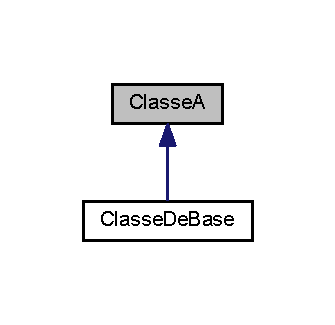
\includegraphics[width=161pt]{class_classe_a__inherit__graph}
\end{center}
\end{figure}
\subsection*{Fonctions membres publiques}
\begin{DoxyCompactItemize}
\item 
void {\bf ajouter\+Composition\+Multiple} ({\bf ptr} nouvel\+Element)
\begin{DoxyCompactList}\small\item\em $<$ Ajouter un élement dans m\+\_\+composition\+Multiple \end{DoxyCompactList}\item 
void {\bf retirer\+Composition\+Multiple} (int id)
\begin{DoxyCompactList}\small\item\em retirer l\textquotesingle{}élement à la position id dans m\+\_\+composition\+Multiple \end{DoxyCompactList}\item 
void {\bf vider\+Composition\+Multiple} ()
\begin{DoxyCompactList}\small\item\em Vider m\+\_\+composition\+Multiple. \end{DoxyCompactList}\item 
{\bf ptr} {\bf get\+Composition\+Multiple} (int id) const 
\begin{DoxyCompactList}\small\item\em Accesseur à l\textquotesingle{}élément de m\+\_\+composition\+Multiple désigné par un id. \end{DoxyCompactList}\item 
bool {\bf operation\+\_\+\+A1} ()
\begin{DoxyCompactList}\small\item\em operation simple \end{DoxyCompactList}\item 
virtual void {\bf operation\+\_\+virtuelle} ()
\begin{DoxyCompactList}\small\item\em operation virtuelle \+: dans Dia\+: polymorphe(virtuelle). \end{DoxyCompactList}\item 
virtual void {\bf operation\+\_\+abstraite} ()=0
\begin{DoxyCompactList}\small\item\em operation abstraite \+: dans Dia\+: Abstraite. Doit etre overridé par héritié. N\textquotesingle{}est par définie dans le $\ast$.cpp. \end{DoxyCompactList}\end{DoxyCompactItemize}
\subsection*{Attributs publics}
\begin{DoxyCompactItemize}
\item 
float {\bf m\+\_\+attr\+\_\+\+A1}
\begin{DoxyCompactList}\small\item\em Attribut direct dans les propriétés de \doxyref{Classe\+A}{p.}{class_classe_a}. \end{DoxyCompactList}\item 
std\+::vector$<$ {\bf ptr} $>$ {\bf m\+\_\+composition\+Multiple}
\begin{DoxyCompactList}\small\item\em multiplicité\+: $\ast$ ou 0..$\ast$ \+: creation vector de cet attribut. En mettant \#\+A, \#\+R, \#\+V, \#\+G dans le commentaire d\textquotesingle{}un vector d\textquotesingle{}attributs on indique a dia2code de prevoir les fonctions ajouter, retirer, vider, get dans le $\ast$.h \end{DoxyCompactList}\end{DoxyCompactItemize}
\subsection*{Types privés}
\begin{DoxyCompactItemize}
\item 
typedef std\+::shared\+\_\+ptr$<$ {\bf Classe\+B} $>$ {\bf ptr}
\begin{DoxyCompactList}\small\item\em Celui ci est integré comme definition de type car la liaison est vide. \end{DoxyCompactList}\end{DoxyCompactItemize}


\subsection{Description détaillée}
Dans la \doxyref{Classe\+A}{p.}{class_classe_a} on colle une définition de type et on utilise ce type dans 2 attributs associés en multiple (dans des vectors ($\ast$) 

\subsection{Documentation des définitions de type membres}
\index{Classe\+A@{Classe\+A}!ptr@{ptr}}
\index{ptr@{ptr}!Classe\+A@{Classe\+A}}
\subsubsection[{ptr}]{\setlength{\rightskip}{0pt plus 5cm}typedef std\+::shared\+\_\+ptr$<${\bf Classe\+B}$>$ {\bf Classe\+A\+::ptr}\hspace{0.3cm}{\ttfamily [private]}}\label{class_classe_a_a459f6871995e0425cc373779acd645bf}


Celui ci est integré comme definition de type car la liaison est vide. 



\subsection{Documentation des fonctions membres}
\index{Classe\+A@{Classe\+A}!ajouter\+Composition\+Multiple@{ajouter\+Composition\+Multiple}}
\index{ajouter\+Composition\+Multiple@{ajouter\+Composition\+Multiple}!Classe\+A@{Classe\+A}}
\subsubsection[{ajouter\+Composition\+Multiple(ptr nouvel\+Element)}]{\setlength{\rightskip}{0pt plus 5cm}void Classe\+A\+::ajouter\+Composition\+Multiple (
\begin{DoxyParamCaption}
\item[{{\bf ptr}}]{nouvel\+Element}
\end{DoxyParamCaption}
)\hspace{0.3cm}{\ttfamily [inline]}}\label{class_classe_a_a5c591b7fa87ba8702ba94870b07a18c2}


$<$ Ajouter un élement dans m\+\_\+composition\+Multiple 

\index{Classe\+A@{Classe\+A}!get\+Composition\+Multiple@{get\+Composition\+Multiple}}
\index{get\+Composition\+Multiple@{get\+Composition\+Multiple}!Classe\+A@{Classe\+A}}
\subsubsection[{get\+Composition\+Multiple(int id) const }]{\setlength{\rightskip}{0pt plus 5cm}{\bf ptr} Classe\+A\+::get\+Composition\+Multiple (
\begin{DoxyParamCaption}
\item[{int}]{id}
\end{DoxyParamCaption}
) const\hspace{0.3cm}{\ttfamily [inline]}}\label{class_classe_a_acdae73528ed6b77d64c67f765a0c052e}


Accesseur à l\textquotesingle{}élément de m\+\_\+composition\+Multiple désigné par un id. 

\index{Classe\+A@{Classe\+A}!operation\+\_\+\+A1@{operation\+\_\+\+A1}}
\index{operation\+\_\+\+A1@{operation\+\_\+\+A1}!Classe\+A@{Classe\+A}}
\subsubsection[{operation\+\_\+\+A1()}]{\setlength{\rightskip}{0pt plus 5cm}bool Classe\+A\+::operation\+\_\+\+A1 (
\begin{DoxyParamCaption}
{}
\end{DoxyParamCaption}
)}\label{class_classe_a_a5457ae6df0159e29191ee5179580717f}


operation simple 

\index{Classe\+A@{Classe\+A}!operation\+\_\+abstraite@{operation\+\_\+abstraite}}
\index{operation\+\_\+abstraite@{operation\+\_\+abstraite}!Classe\+A@{Classe\+A}}
\subsubsection[{operation\+\_\+abstraite()=0}]{\setlength{\rightskip}{0pt plus 5cm}virtual void Classe\+A\+::operation\+\_\+abstraite (
\begin{DoxyParamCaption}
{}
\end{DoxyParamCaption}
)\hspace{0.3cm}{\ttfamily [pure virtual]}}\label{class_classe_a_a0aa4415d54ac490c633a3bb15fc54d50}


operation abstraite \+: dans Dia\+: Abstraite. Doit etre overridé par héritié. N\textquotesingle{}est par définie dans le $\ast$.cpp. 



Implémenté dans {\bf Classe\+De\+Base} \doxyref{}{p.}{class_classe_de_base_a066806c67b8ae57e247992dcd905dd9e}.

\index{Classe\+A@{Classe\+A}!operation\+\_\+virtuelle@{operation\+\_\+virtuelle}}
\index{operation\+\_\+virtuelle@{operation\+\_\+virtuelle}!Classe\+A@{Classe\+A}}
\subsubsection[{operation\+\_\+virtuelle()}]{\setlength{\rightskip}{0pt plus 5cm}void Classe\+A\+::operation\+\_\+virtuelle (
\begin{DoxyParamCaption}
{}
\end{DoxyParamCaption}
)\hspace{0.3cm}{\ttfamily [virtual]}}\label{class_classe_a_a7d34e699687795ee47a2da2ab89fd7c2}


operation virtuelle \+: dans Dia\+: polymorphe(virtuelle). 



Réimplémentée dans {\bf Classe\+De\+Base} \doxyref{}{p.}{class_classe_de_base_a69c1bbd18ee2f1989141443328dcd031}.

\index{Classe\+A@{Classe\+A}!retirer\+Composition\+Multiple@{retirer\+Composition\+Multiple}}
\index{retirer\+Composition\+Multiple@{retirer\+Composition\+Multiple}!Classe\+A@{Classe\+A}}
\subsubsection[{retirer\+Composition\+Multiple(int id)}]{\setlength{\rightskip}{0pt plus 5cm}void Classe\+A\+::retirer\+Composition\+Multiple (
\begin{DoxyParamCaption}
\item[{int}]{id}
\end{DoxyParamCaption}
)\hspace{0.3cm}{\ttfamily [inline]}}\label{class_classe_a_a5c1a45ab82ee8d64c0bc44605596b604}


retirer l\textquotesingle{}élement à la position id dans m\+\_\+composition\+Multiple 

\index{Classe\+A@{Classe\+A}!vider\+Composition\+Multiple@{vider\+Composition\+Multiple}}
\index{vider\+Composition\+Multiple@{vider\+Composition\+Multiple}!Classe\+A@{Classe\+A}}
\subsubsection[{vider\+Composition\+Multiple()}]{\setlength{\rightskip}{0pt plus 5cm}void Classe\+A\+::vider\+Composition\+Multiple (
\begin{DoxyParamCaption}
{}
\end{DoxyParamCaption}
)\hspace{0.3cm}{\ttfamily [inline]}}\label{class_classe_a_a7422a682f9976d916b96ccf49ea6b2ee}


Vider m\+\_\+composition\+Multiple. 



\subsection{Documentation des données membres}
\index{Classe\+A@{Classe\+A}!m\+\_\+attr\+\_\+\+A1@{m\+\_\+attr\+\_\+\+A1}}
\index{m\+\_\+attr\+\_\+\+A1@{m\+\_\+attr\+\_\+\+A1}!Classe\+A@{Classe\+A}}
\subsubsection[{m\+\_\+attr\+\_\+\+A1}]{\setlength{\rightskip}{0pt plus 5cm}float Classe\+A\+::m\+\_\+attr\+\_\+\+A1}\label{class_classe_a_acff950594aaeae758faca3a7d114aa32}


Attribut direct dans les propriétés de \doxyref{Classe\+A}{p.}{class_classe_a}. 

\index{Classe\+A@{Classe\+A}!m\+\_\+composition\+Multiple@{m\+\_\+composition\+Multiple}}
\index{m\+\_\+composition\+Multiple@{m\+\_\+composition\+Multiple}!Classe\+A@{Classe\+A}}
\subsubsection[{m\+\_\+composition\+Multiple}]{\setlength{\rightskip}{0pt plus 5cm}std\+::vector$<${\bf ptr}$>$ Classe\+A\+::m\+\_\+composition\+Multiple}\label{class_classe_a_adb7b2ed3211a7950b544d7ae4fb0af45}


multiplicité\+: $\ast$ ou 0..$\ast$ \+: creation vector de cet attribut. En mettant \#\+A, \#\+R, \#\+V, \#\+G dans le commentaire d\textquotesingle{}un vector d\textquotesingle{}attributs on indique a dia2code de prevoir les fonctions ajouter, retirer, vider, get dans le $\ast$.h 



La documentation de cette classe a été générée à partir des fichiers suivants \+:\begin{DoxyCompactItemize}
\item 
R\+:/06 -\/ C++/dia2code\+Perso/exemple/code\+C\+P\+P\+\_\+exemple 0/include/{\bf Classe\+A.\+h}\item 
R\+:/06 -\/ C++/dia2code\+Perso/exemple/code\+C\+P\+P\+\_\+exemple 0/src/{\bf Classe\+A.\+cpp}\end{DoxyCompactItemize}

\section{Référence de la classe Classe\+B}
\label{class_classe_b}\index{Classe\+B@{Classe\+B}}


associé avec le type\+: \textquotesingle{}Aggregation\textquotesingle{}. Créer l\textquotesingle{}attribut dans un shared\+\_\+ptr.  




{\ttfamily \#include $<$Classe\+B.\+h$>$}

\subsection*{Fonctions membres publiques}
\begin{DoxyCompactItemize}
\item 
bool {\bf operation\+\_\+\+B1} ()
\begin{DoxyCompactList}\small\item\em operation simple \end{DoxyCompactList}\end{DoxyCompactItemize}
\subsection*{Attributs publics}
\begin{DoxyCompactItemize}
\item 
sf\+::\+Float\+Rect {\bf m\+\_\+\+Truc\+S\+F\+M\+L}
\begin{DoxyCompactList}\small\item\em Un peu tricky \+: le type comprte \char`\"{}sf\+::\char`\"{} on include donc $<$S\+F\+M\+L/\+Graphics.\+hpp$>$. \end{DoxyCompactList}\item 
std\+::shared\+\_\+ptr$<$ {\bf Classe\+C} $>$ {\bf m\+\_\+classe\+C}
\begin{DoxyCompactList}\small\item\em ceci ajoute l\textquotesingle{}include $<$memory$>$, definie temporairement la Class\+C dans le $\ast$.h, et include \doxyref{Classe\+C}{p.}{class_classe_c} dans le $\ast$.cpp. \end{DoxyCompactList}\item 
float {\bf m\+\_\+attr\+\_\+\+B1}
\begin{DoxyCompactList}\small\item\em Attribut direct dans les propriétés de \doxyref{Classe\+B}{p.}{class_classe_b}. \end{DoxyCompactList}\end{DoxyCompactItemize}


\subsection{Description détaillée}
associé avec le type\+: \textquotesingle{}Aggregation\textquotesingle{}. Créer l\textquotesingle{}attribut dans un shared\+\_\+ptr. 

\subsection{Documentation des fonctions membres}
\index{Classe\+B@{Classe\+B}!operation\+\_\+\+B1@{operation\+\_\+\+B1}}
\index{operation\+\_\+\+B1@{operation\+\_\+\+B1}!Classe\+B@{Classe\+B}}
\subsubsection[{operation\+\_\+\+B1()}]{\setlength{\rightskip}{0pt plus 5cm}bool Classe\+B\+::operation\+\_\+\+B1 (
\begin{DoxyParamCaption}
{}
\end{DoxyParamCaption}
)}\label{class_classe_b_a4a2e82d68664a57ad9f922543e2eed18}


operation simple 



\subsection{Documentation des données membres}
\index{Classe\+B@{Classe\+B}!m\+\_\+attr\+\_\+\+B1@{m\+\_\+attr\+\_\+\+B1}}
\index{m\+\_\+attr\+\_\+\+B1@{m\+\_\+attr\+\_\+\+B1}!Classe\+B@{Classe\+B}}
\subsubsection[{m\+\_\+attr\+\_\+\+B1}]{\setlength{\rightskip}{0pt plus 5cm}float Classe\+B\+::m\+\_\+attr\+\_\+\+B1}\label{class_classe_b_a3db1ea15c88b64e3e428e2b22416af39}


Attribut direct dans les propriétés de \doxyref{Classe\+B}{p.}{class_classe_b}. 

\index{Classe\+B@{Classe\+B}!m\+\_\+classe\+C@{m\+\_\+classe\+C}}
\index{m\+\_\+classe\+C@{m\+\_\+classe\+C}!Classe\+B@{Classe\+B}}
\subsubsection[{m\+\_\+classe\+C}]{\setlength{\rightskip}{0pt plus 5cm}std\+::shared\+\_\+ptr$<${\bf Classe\+C}$>$ Classe\+B\+::m\+\_\+classe\+C}\label{class_classe_b_ad3e8fc2038d1aebf65a7a0df2bb4fc78}


ceci ajoute l\textquotesingle{}include $<$memory$>$, definie temporairement la Class\+C dans le $\ast$.h, et include \doxyref{Classe\+C}{p.}{class_classe_c} dans le $\ast$.cpp. 

\index{Classe\+B@{Classe\+B}!m\+\_\+\+Truc\+S\+F\+M\+L@{m\+\_\+\+Truc\+S\+F\+M\+L}}
\index{m\+\_\+\+Truc\+S\+F\+M\+L@{m\+\_\+\+Truc\+S\+F\+M\+L}!Classe\+B@{Classe\+B}}
\subsubsection[{m\+\_\+\+Truc\+S\+F\+M\+L}]{\setlength{\rightskip}{0pt plus 5cm}sf\+::\+Float\+Rect Classe\+B\+::m\+\_\+\+Truc\+S\+F\+M\+L}\label{class_classe_b_a23514f02a80438f4ea56e8dfc6efbdfd}


Un peu tricky \+: le type comprte \char`\"{}sf\+::\char`\"{} on include donc $<$S\+F\+M\+L/\+Graphics.\+hpp$>$. 



La documentation de cette classe a été générée à partir des fichiers suivants \+:\begin{DoxyCompactItemize}
\item 
R\+:/06 -\/ C++/dia2code\+Perso/exemple/code\+C\+P\+P\+\_\+exemple 0/include/{\bf Classe\+B.\+h}\item 
R\+:/06 -\/ C++/dia2code\+Perso/exemple/code\+C\+P\+P\+\_\+exemple 0/src/{\bf Classe\+B.\+cpp}\end{DoxyCompactItemize}

\section{Référence de la classe Classe\+C}
\label{class_classe_c}\index{Classe\+C@{Classe\+C}}


ici on associe 2 stereotypes \+: un using et un enum  




{\ttfamily \#include $<$Classe\+C.\+h$>$}



Graphe d\textquotesingle{}héritage de Classe\+C\+:
\nopagebreak
\begin{figure}[H]
\begin{center}
\leavevmode
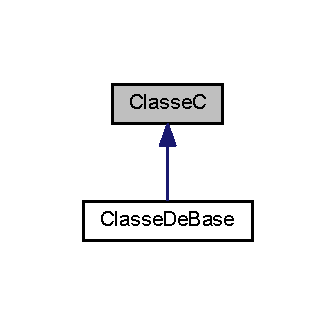
\includegraphics[width=161pt]{class_classe_c__inherit__graph}
\end{center}
\end{figure}
\subsection*{Fonctions membres publiques}
\begin{DoxyCompactItemize}
\item 
bool {\bf operation\+\_\+\+C1} ()
\begin{DoxyCompactList}\small\item\em operation simple \end{DoxyCompactList}\item 
float {\bf get\+\_\+attr\+\_\+\+C1} () const 
\begin{DoxyCompactList}\small\item\em Accesseur de l\textquotesingle{}attribut C1, c\textquotesingle{}est une requête, \textquotesingle{}const\textquotesingle{} sera ajouté dans le $\ast$.h. \end{DoxyCompactList}\end{DoxyCompactItemize}
\subsection*{Attributs publics}
\begin{DoxyCompactItemize}
\item 
float {\bf m\+\_\+attr\+\_\+\+C1}
\begin{DoxyCompactList}\small\item\em Attribut direct dans les propriétés de \doxyref{Classe\+C}{p.}{class_classe_c}. \end{DoxyCompactList}\item 
std\+::vector$<$ {\bf Classe\+A} $>$ {\bf m\+\_\+vect\+Attribut\+\_\+\+C1}
\begin{DoxyCompactList}\small\item\em Ceci inclus $<$vector$>$ et déclare \doxyref{Classe\+A}{p.}{class_classe_a}. \end{DoxyCompactList}\end{DoxyCompactItemize}
\subsection*{Types privés}
\begin{DoxyCompactItemize}
\item 
enum {\bf Enum\+C} \{ {\bf enum1}, 
{\bf enum2}, 
{\bf enum3}
 \}\begin{DoxyCompactList}\small\item\em Un exemple d\textquotesingle{}integration du stereotype $<$$<$enum$>$$>$. Chaque élément de l\textquotesingle{}énumération est stocké dans le Nom d\textquotesingle{}un attribut. \end{DoxyCompactList}
\item 
using {\bf Fctn\+Action} = std\+::function$<$ void()$>$
\begin{DoxyCompactList}\small\item\em Un exemple d\textquotesingle{}integration du stereotype $<$$<$using$>$$>$ avec l\textquotesingle{}include de $<$function$>$ \end{DoxyCompactList}\end{DoxyCompactItemize}


\subsection{Description détaillée}
ici on associe 2 stereotypes \+: un using et un enum 

\subsection{Documentation des définitions de type membres}
\index{Classe\+C@{Classe\+C}!Fctn\+Action@{Fctn\+Action}}
\index{Fctn\+Action@{Fctn\+Action}!Classe\+C@{Classe\+C}}
\subsubsection[{Fctn\+Action}]{\setlength{\rightskip}{0pt plus 5cm}using {\bf Classe\+C\+::\+Fctn\+Action} =  std\+::function$<$void()$>$\hspace{0.3cm}{\ttfamily [private]}}\label{class_classe_c_a14817d34592f1e30f6ee61f8a829e8ab}


Un exemple d\textquotesingle{}integration du stereotype $<$$<$using$>$$>$ avec l\textquotesingle{}include de $<$function$>$ 



\subsection{Documentation des énumérations membres}
\index{Classe\+C@{Classe\+C}!Enum\+C@{Enum\+C}}
\index{Enum\+C@{Enum\+C}!Classe\+C@{Classe\+C}}
\subsubsection[{Enum\+C}]{\setlength{\rightskip}{0pt plus 5cm}enum {\bf Classe\+C\+::\+Enum\+C}\hspace{0.3cm}{\ttfamily [private]}}\label{class_classe_c_a4d59a03daacbc085bea317ceb30fdc88}


Un exemple d\textquotesingle{}integration du stereotype $<$$<$enum$>$$>$. Chaque élément de l\textquotesingle{}énumération est stocké dans le Nom d\textquotesingle{}un attribut. 

\begin{Desc}
\item[Valeurs énumérées]\par
\begin{description}
\index{enum1@{enum1}!Classe\+C@{Classe\+C}}\index{Classe\+C@{Classe\+C}!enum1@{enum1}}\item[{\em 
enum1\label{class_classe_c_a4d59a03daacbc085bea317ceb30fdc88a6cf42a63ad24d65ce659d67c1c2c9c4d}
}]Commentaire de l\textquotesingle{}enum 1. \index{enum2@{enum2}!Classe\+C@{Classe\+C}}\index{Classe\+C@{Classe\+C}!enum2@{enum2}}\item[{\em 
enum2\label{class_classe_c_a4d59a03daacbc085bea317ceb30fdc88a0241a8ac8b0278431e63cd82e9a643c3}
}]Commentaire de l\textquotesingle{}enum 2. \index{enum3@{enum3}!Classe\+C@{Classe\+C}}\index{Classe\+C@{Classe\+C}!enum3@{enum3}}\item[{\em 
enum3\label{class_classe_c_a4d59a03daacbc085bea317ceb30fdc88afa5ff07577a7a59f1baf77d2fa6f1aa1}
}]Commentaire de l\textquotesingle{}enum 3. \end{description}
\end{Desc}


\subsection{Documentation des fonctions membres}
\index{Classe\+C@{Classe\+C}!get\+\_\+attr\+\_\+\+C1@{get\+\_\+attr\+\_\+\+C1}}
\index{get\+\_\+attr\+\_\+\+C1@{get\+\_\+attr\+\_\+\+C1}!Classe\+C@{Classe\+C}}
\subsubsection[{get\+\_\+attr\+\_\+\+C1() const }]{\setlength{\rightskip}{0pt plus 5cm}float Classe\+C\+::get\+\_\+attr\+\_\+\+C1 (
\begin{DoxyParamCaption}
{}
\end{DoxyParamCaption}
) const}\label{class_classe_c_a8de2d661dce321d77ab319860e8bc6fa}


Accesseur de l\textquotesingle{}attribut C1, c\textquotesingle{}est une requête, \textquotesingle{}const\textquotesingle{} sera ajouté dans le $\ast$.h. 

\index{Classe\+C@{Classe\+C}!operation\+\_\+\+C1@{operation\+\_\+\+C1}}
\index{operation\+\_\+\+C1@{operation\+\_\+\+C1}!Classe\+C@{Classe\+C}}
\subsubsection[{operation\+\_\+\+C1()}]{\setlength{\rightskip}{0pt plus 5cm}bool Classe\+C\+::operation\+\_\+\+C1 (
\begin{DoxyParamCaption}
{}
\end{DoxyParamCaption}
)}\label{class_classe_c_a3c6604c135751f5580afb6f9aad50592}


operation simple 



\subsection{Documentation des données membres}
\index{Classe\+C@{Classe\+C}!m\+\_\+attr\+\_\+\+C1@{m\+\_\+attr\+\_\+\+C1}}
\index{m\+\_\+attr\+\_\+\+C1@{m\+\_\+attr\+\_\+\+C1}!Classe\+C@{Classe\+C}}
\subsubsection[{m\+\_\+attr\+\_\+\+C1}]{\setlength{\rightskip}{0pt plus 5cm}float Classe\+C\+::m\+\_\+attr\+\_\+\+C1}\label{class_classe_c_afe4145c8d88c974672845e496edd761d}


Attribut direct dans les propriétés de \doxyref{Classe\+C}{p.}{class_classe_c}. 

\index{Classe\+C@{Classe\+C}!m\+\_\+vect\+Attribut\+\_\+\+C1@{m\+\_\+vect\+Attribut\+\_\+\+C1}}
\index{m\+\_\+vect\+Attribut\+\_\+\+C1@{m\+\_\+vect\+Attribut\+\_\+\+C1}!Classe\+C@{Classe\+C}}
\subsubsection[{m\+\_\+vect\+Attribut\+\_\+\+C1}]{\setlength{\rightskip}{0pt plus 5cm}std\+::vector$<${\bf Classe\+A}$>$ Classe\+C\+::m\+\_\+vect\+Attribut\+\_\+\+C1}\label{class_classe_c_aa86493beaa3a115e86cfd67346f73d44}


Ceci inclus $<$vector$>$ et déclare \doxyref{Classe\+A}{p.}{class_classe_a}. 



La documentation de cette classe a été générée à partir des fichiers suivants \+:\begin{DoxyCompactItemize}
\item 
R\+:/06 -\/ C++/dia2code\+Perso/exemple/code\+C\+P\+P\+\_\+exemple 0/include/{\bf Classe\+C.\+h}\item 
R\+:/06 -\/ C++/dia2code\+Perso/exemple/code\+C\+P\+P\+\_\+exemple 0/src/{\bf Classe\+C.\+cpp}\end{DoxyCompactItemize}

\section{Référence de la classe Classe\+De\+Base}
\label{class_classe_de_base}\index{Classe\+De\+Base@{Classe\+De\+Base}}


Classe qui hérite de 2 autres classes. Cela ajoutera les includes necéssaires.  




{\ttfamily \#include $<$Classe\+De\+Base.\+h$>$}



Graphe d\textquotesingle{}héritage de Classe\+De\+Base\+:\nopagebreak
\begin{figure}[H]
\begin{center}
\leavevmode
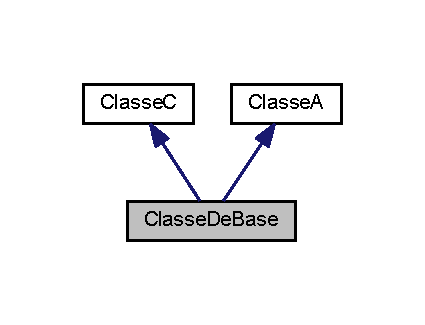
\includegraphics[width=204pt]{class_classe_de_base__inherit__graph}
\end{center}
\end{figure}


Graphe de collaboration de Classe\+De\+Base\+:
\nopagebreak
\begin{figure}[H]
\begin{center}
\leavevmode
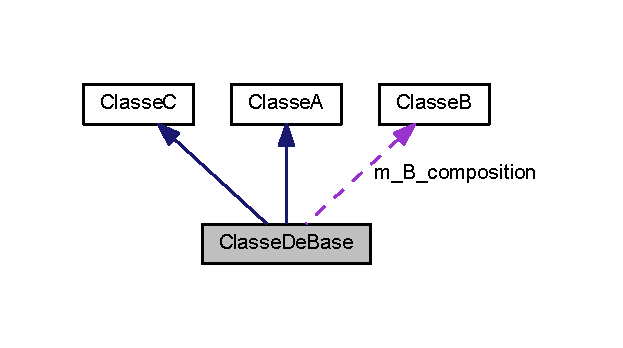
\includegraphics[width=287pt]{class_classe_de_base__coll__graph}
\end{center}
\end{figure}
\subsection*{Fonctions membres publiques}
\begin{DoxyCompactItemize}
\item 
void {\bf set\+Composition} ({\bf Classe\+B} val)
\begin{DoxyCompactList}\small\item\em $<$ Definir m\+\_\+composition \end{DoxyCompactList}\item 
{\bf Classe\+B} {\bf get\+Composition} () const 
\begin{DoxyCompactList}\small\item\em Acceder à m\+\_\+composition. \end{DoxyCompactList}\item 
void {\bf set\+Aggregation} (std\+::shared\+\_\+ptr$<$ {\bf Classe\+B} $>$ val)
\begin{DoxyCompactList}\small\item\em Definir m\+\_\+aggregation. \end{DoxyCompactList}\item 
std\+::shared\+\_\+ptr$<$ {\bf Classe\+B} $>$ {\bf get\+Aggregation} () const 
\begin{DoxyCompactList}\small\item\em Acceder à m\+\_\+aggregation. \end{DoxyCompactList}\item 
{\bf Classe\+De\+Base} ()
\begin{DoxyCompactList}\small\item\em Constructeur, les attributs ayant une valeur par défaut vont être initialisés dans le $\ast$.cpp. \end{DoxyCompactList}\item 
void {\bf operation\+\_\+1} (int param1)
\begin{DoxyCompactList}\small\item\em operation public de base. \end{DoxyCompactList}\item 
virtual void {\bf operation\+\_\+virtuelle} ()
\begin{DoxyCompactList}\small\item\em operation virtuelle qui override celle de la \doxyref{Classe\+A}{p.}{class_classe_a}. \end{DoxyCompactList}\item 
virtual void {\bf operation\+\_\+abstraite} ()
\begin{DoxyCompactList}\small\item\em operation virtuelle qui override l\textquotesingle{}operation abstraite de la \doxyref{Classe\+A}{p.}{class_classe_a}. \end{DoxyCompactList}\end{DoxyCompactItemize}
\subsection*{Attributs publics}
\begin{DoxyCompactItemize}
\item 
int {\bf m\+\_\+attr\+\_\+2}
\begin{DoxyCompactList}\small\item\em Attribut public de la classe de base. \end{DoxyCompactList}\end{DoxyCompactItemize}
\subsection*{Attributs publics statiques}
\begin{DoxyCompactItemize}
\item 
static int {\bf ms\+\_\+attr\+\_\+1} = 0
\begin{DoxyCompactList}\small\item\em Attribut static de la classe de base. Sera initialisé au début du $\ast$.cpp. \end{DoxyCompactList}\end{DoxyCompactItemize}
\subsection*{Attributs protégés}
\begin{DoxyCompactItemize}
\item 
int {\bf m\+\_\+attr\+\_\+3}
\begin{DoxyCompactList}\small\item\em Attribut protegé de la classe de base. \end{DoxyCompactList}\item 
{\bf Classe\+B} {\bf m\+\_\+composition}
\begin{DoxyCompactList}\small\item\em associé avec le type\+: \textquotesingle{}composition\textquotesingle{}, créer un simple attribut. \#\+G\#\+S \end{DoxyCompactList}\item 
std\+::shared\+\_\+ptr$<$ {\bf Classe\+B} $>$ {\bf m\+\_\+aggregation}
\begin{DoxyCompactList}\small\item\em associé avec le type\+: \textquotesingle{}Aggregation\textquotesingle{}. Créer l\textquotesingle{}attribut dans un shared\+\_\+ptr. En mettant \#\+G ou \#\+S dans le commentaire d\textquotesingle{}un attribut on indique a dia2code de prevoir les fonctions get ou set dans le $\ast$.h. \end{DoxyCompactList}\end{DoxyCompactItemize}


\subsection{Description détaillée}
Classe qui hérite de 2 autres classes. Cela ajoutera les includes necéssaires. 

\subsection{Documentation des constructeurs et destructeur}
\index{Classe\+De\+Base@{Classe\+De\+Base}!Classe\+De\+Base@{Classe\+De\+Base}}
\index{Classe\+De\+Base@{Classe\+De\+Base}!Classe\+De\+Base@{Classe\+De\+Base}}
\subsubsection[{Classe\+De\+Base()}]{\setlength{\rightskip}{0pt plus 5cm}Classe\+De\+Base\+::\+Classe\+De\+Base (
\begin{DoxyParamCaption}
{}
\end{DoxyParamCaption}
)}\label{class_classe_de_base_ab12f84aa56a394fa0f7db9518af68f70}


Constructeur, les attributs ayant une valeur par défaut vont être initialisés dans le $\ast$.cpp. 



\subsection{Documentation des fonctions membres}
\index{Classe\+De\+Base@{Classe\+De\+Base}!get\+Aggregation@{get\+Aggregation}}
\index{get\+Aggregation@{get\+Aggregation}!Classe\+De\+Base@{Classe\+De\+Base}}
\subsubsection[{get\+Aggregation() const }]{\setlength{\rightskip}{0pt plus 5cm}std\+::shared\+\_\+ptr$<${\bf Classe\+B}$>$ Classe\+De\+Base\+::get\+Aggregation (
\begin{DoxyParamCaption}
{}
\end{DoxyParamCaption}
) const\hspace{0.3cm}{\ttfamily [inline]}}\label{class_classe_de_base_adfc900acc95b173c17858c8c62f94507}


Acceder à m\+\_\+aggregation. 

\index{Classe\+De\+Base@{Classe\+De\+Base}!get\+Composition@{get\+Composition}}
\index{get\+Composition@{get\+Composition}!Classe\+De\+Base@{Classe\+De\+Base}}
\subsubsection[{get\+Composition() const }]{\setlength{\rightskip}{0pt plus 5cm}{\bf Classe\+B} Classe\+De\+Base\+::get\+Composition (
\begin{DoxyParamCaption}
{}
\end{DoxyParamCaption}
) const\hspace{0.3cm}{\ttfamily [inline]}}\label{class_classe_de_base_aa389d39667d11658acdbe4e0011d2f6d}


Acceder à m\+\_\+composition. 

\index{Classe\+De\+Base@{Classe\+De\+Base}!operation\+\_\+1@{operation\+\_\+1}}
\index{operation\+\_\+1@{operation\+\_\+1}!Classe\+De\+Base@{Classe\+De\+Base}}
\subsubsection[{operation\+\_\+1(int param1)}]{\setlength{\rightskip}{0pt plus 5cm}void Classe\+De\+Base\+::operation\+\_\+1 (
\begin{DoxyParamCaption}
\item[{int}]{param1}
\end{DoxyParamCaption}
)}\label{class_classe_de_base_a1e6d89bbc396d801afddc4f7bc715537}


operation public de base. 


\begin{DoxyParams}{Paramètres}
{\em param1} & Parametre de l\textquotesingle{}operation. \\
\hline
\end{DoxyParams}
\index{Classe\+De\+Base@{Classe\+De\+Base}!operation\+\_\+abstraite@{operation\+\_\+abstraite}}
\index{operation\+\_\+abstraite@{operation\+\_\+abstraite}!Classe\+De\+Base@{Classe\+De\+Base}}
\subsubsection[{operation\+\_\+abstraite()}]{\setlength{\rightskip}{0pt plus 5cm}void Classe\+De\+Base\+::operation\+\_\+abstraite (
\begin{DoxyParamCaption}
{}
\end{DoxyParamCaption}
)\hspace{0.3cm}{\ttfamily [virtual]}}\label{class_classe_de_base_a066806c67b8ae57e247992dcd905dd9e}


operation virtuelle qui override l\textquotesingle{}operation abstraite de la \doxyref{Classe\+A}{p.}{class_classe_a}. 



Implémente {\bf Classe\+A} \doxyref{}{p.}{class_classe_a_a0aa4415d54ac490c633a3bb15fc54d50}.

\index{Classe\+De\+Base@{Classe\+De\+Base}!operation\+\_\+virtuelle@{operation\+\_\+virtuelle}}
\index{operation\+\_\+virtuelle@{operation\+\_\+virtuelle}!Classe\+De\+Base@{Classe\+De\+Base}}
\subsubsection[{operation\+\_\+virtuelle()}]{\setlength{\rightskip}{0pt plus 5cm}void Classe\+De\+Base\+::operation\+\_\+virtuelle (
\begin{DoxyParamCaption}
{}
\end{DoxyParamCaption}
)\hspace{0.3cm}{\ttfamily [virtual]}}\label{class_classe_de_base_a69c1bbd18ee2f1989141443328dcd031}


operation virtuelle qui override celle de la \doxyref{Classe\+A}{p.}{class_classe_a}. 



Réimplémentée à partir de {\bf Classe\+A} \doxyref{}{p.}{class_classe_a_a7d34e699687795ee47a2da2ab89fd7c2}.

\index{Classe\+De\+Base@{Classe\+De\+Base}!set\+Aggregation@{set\+Aggregation}}
\index{set\+Aggregation@{set\+Aggregation}!Classe\+De\+Base@{Classe\+De\+Base}}
\subsubsection[{set\+Aggregation(std\+::shared\+\_\+ptr$<$ Classe\+B $>$ val)}]{\setlength{\rightskip}{0pt plus 5cm}void Classe\+De\+Base\+::set\+Aggregation (
\begin{DoxyParamCaption}
\item[{std\+::shared\+\_\+ptr$<$ {\bf Classe\+B} $>$}]{val}
\end{DoxyParamCaption}
)\hspace{0.3cm}{\ttfamily [inline]}}\label{class_classe_de_base_a8eef736e6fe6de1489350a1802bddf0c}


Definir m\+\_\+aggregation. 

\index{Classe\+De\+Base@{Classe\+De\+Base}!set\+Composition@{set\+Composition}}
\index{set\+Composition@{set\+Composition}!Classe\+De\+Base@{Classe\+De\+Base}}
\subsubsection[{set\+Composition(\+Classe\+B val)}]{\setlength{\rightskip}{0pt plus 5cm}void Classe\+De\+Base\+::set\+Composition (
\begin{DoxyParamCaption}
\item[{{\bf Classe\+B}}]{val}
\end{DoxyParamCaption}
)\hspace{0.3cm}{\ttfamily [inline]}}\label{class_classe_de_base_a3b97aa015ca6c659f1814129f38c8184}


$<$ Definir m\+\_\+composition 



\subsection{Documentation des données membres}
\index{Classe\+De\+Base@{Classe\+De\+Base}!m\+\_\+aggregation@{m\+\_\+aggregation}}
\index{m\+\_\+aggregation@{m\+\_\+aggregation}!Classe\+De\+Base@{Classe\+De\+Base}}
\subsubsection[{m\+\_\+aggregation}]{\setlength{\rightskip}{0pt plus 5cm}std\+::shared\+\_\+ptr$<${\bf Classe\+B}$>$ Classe\+De\+Base\+::m\+\_\+aggregation\hspace{0.3cm}{\ttfamily [protected]}}\label{class_classe_de_base_af579b7e00abce1542661ce59e0894f4a}


associé avec le type\+: \textquotesingle{}Aggregation\textquotesingle{}. Créer l\textquotesingle{}attribut dans un shared\+\_\+ptr. En mettant \#\+G ou \#\+S dans le commentaire d\textquotesingle{}un attribut on indique a dia2code de prevoir les fonctions get ou set dans le $\ast$.h. 

\index{Classe\+De\+Base@{Classe\+De\+Base}!m\+\_\+attr\+\_\+2@{m\+\_\+attr\+\_\+2}}
\index{m\+\_\+attr\+\_\+2@{m\+\_\+attr\+\_\+2}!Classe\+De\+Base@{Classe\+De\+Base}}
\subsubsection[{m\+\_\+attr\+\_\+2}]{\setlength{\rightskip}{0pt plus 5cm}int Classe\+De\+Base\+::m\+\_\+attr\+\_\+2}\label{class_classe_de_base_a8ae3ec3194396062a58f0c953dd9d751}


Attribut public de la classe de base. 

\index{Classe\+De\+Base@{Classe\+De\+Base}!m\+\_\+attr\+\_\+3@{m\+\_\+attr\+\_\+3}}
\index{m\+\_\+attr\+\_\+3@{m\+\_\+attr\+\_\+3}!Classe\+De\+Base@{Classe\+De\+Base}}
\subsubsection[{m\+\_\+attr\+\_\+3}]{\setlength{\rightskip}{0pt plus 5cm}int Classe\+De\+Base\+::m\+\_\+attr\+\_\+3\hspace{0.3cm}{\ttfamily [protected]}}\label{class_classe_de_base_add64a038fee30008edf9b5e7d8e822ea}


Attribut protegé de la classe de base. 

\index{Classe\+De\+Base@{Classe\+De\+Base}!m\+\_\+composition@{m\+\_\+composition}}
\index{m\+\_\+composition@{m\+\_\+composition}!Classe\+De\+Base@{Classe\+De\+Base}}
\subsubsection[{m\+\_\+composition}]{\setlength{\rightskip}{0pt plus 5cm}{\bf Classe\+B} Classe\+De\+Base\+::m\+\_\+composition\hspace{0.3cm}{\ttfamily [protected]}}\label{class_classe_de_base_abc903823f6013670eb5e36676879330e}


associé avec le type\+: \textquotesingle{}composition\textquotesingle{}, créer un simple attribut. \#\+G\#\+S 

\index{Classe\+De\+Base@{Classe\+De\+Base}!ms\+\_\+attr\+\_\+1@{ms\+\_\+attr\+\_\+1}}
\index{ms\+\_\+attr\+\_\+1@{ms\+\_\+attr\+\_\+1}!Classe\+De\+Base@{Classe\+De\+Base}}
\subsubsection[{ms\+\_\+attr\+\_\+1}]{\setlength{\rightskip}{0pt plus 5cm}int Classe\+De\+Base\+::ms\+\_\+attr\+\_\+1 = 0\hspace{0.3cm}{\ttfamily [static]}}\label{class_classe_de_base_a052532b7d64e18455fbf76d405b882a7}


Attribut static de la classe de base. Sera initialisé au début du $\ast$.cpp. 



La documentation de cette classe a été générée à partir des fichiers suivants \+:\begin{DoxyCompactItemize}
\item 
R\+:/06 -\/ C++/dia2code\+Perso/exemple/code\+C\+P\+P\+\_\+exemple 0/include/{\bf Classe\+De\+Base.\+h}\item 
R\+:/06 -\/ C++/dia2code\+Perso/exemple/code\+C\+P\+P\+\_\+exemple 0/src/{\bf Classe\+De\+Base.\+cpp}\end{DoxyCompactItemize}

\chapter{Documentation des fichiers}
\section{Référence du fichier R\+:/06 -\/ C++/dia2code\+Perso/exemple/code\+C\+P\+P\+\_\+exemple 0/include/\+Classe\+A.h}
\label{_classe_a_8h}\index{R\+:/06 -\/ C++/dia2code\+Perso/exemple/code\+C\+P\+P\+\_\+exemple 0/include/\+Classe\+A.\+h@{R\+:/06 -\/ C++/dia2code\+Perso/exemple/code\+C\+P\+P\+\_\+exemple 0/include/\+Classe\+A.\+h}}
{\ttfamily \#include $<$memory$>$}\\*
{\ttfamily \#include $<$vector$>$}\\*
Graphe des dépendances par inclusion de Classe\+A.\+h\+:\nopagebreak
\begin{figure}[H]
\begin{center}
\leavevmode
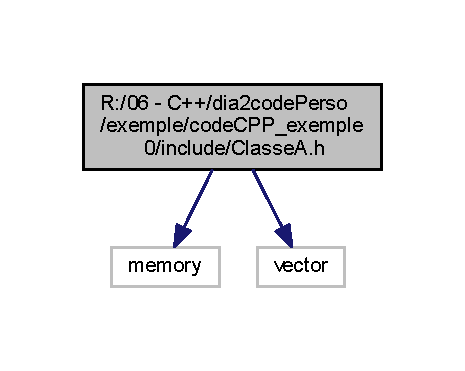
\includegraphics[width=223pt]{_classe_a_8h__incl}
\end{center}
\end{figure}
Ce graphe montre quels fichiers incluent directement ou indirectement ce fichier \+:\nopagebreak
\begin{figure}[H]
\begin{center}
\leavevmode
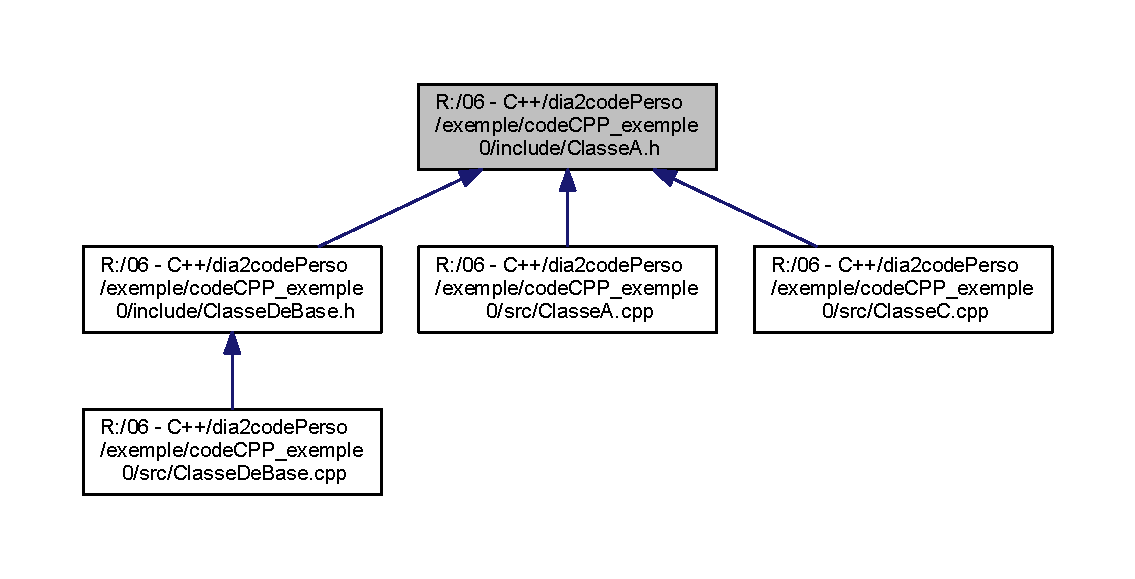
\includegraphics[width=350pt]{_classe_a_8h__dep__incl}
\end{center}
\end{figure}
\subsection*{Classes}
\begin{DoxyCompactItemize}
\item 
class {\bf Classe\+A}
\begin{DoxyCompactList}\small\item\em Dans la \doxyref{Classe\+A}{p.}{class_classe_a} on colle une définition de type et on utilise ce type dans 2 attributs associés en multiple (dans des vectors ($\ast$) \end{DoxyCompactList}\end{DoxyCompactItemize}

\section{Référence du fichier R\+:/06 -\/ C++/dia2code\+Perso/exemple/code\+C\+P\+P\+\_\+exemple 0/include/\+Classe\+B.h}
\label{_classe_b_8h}\index{R\+:/06 -\/ C++/dia2code\+Perso/exemple/code\+C\+P\+P\+\_\+exemple 0/include/\+Classe\+B.\+h@{R\+:/06 -\/ C++/dia2code\+Perso/exemple/code\+C\+P\+P\+\_\+exemple 0/include/\+Classe\+B.\+h}}
{\ttfamily \#include $<$S\+F\+M\+L/\+Graphics.\+hpp$>$}\\*
{\ttfamily \#include $<$memory$>$}\\*
Graphe des dépendances par inclusion de Classe\+B.\+h\+:
\nopagebreak
\begin{figure}[H]
\begin{center}
\leavevmode
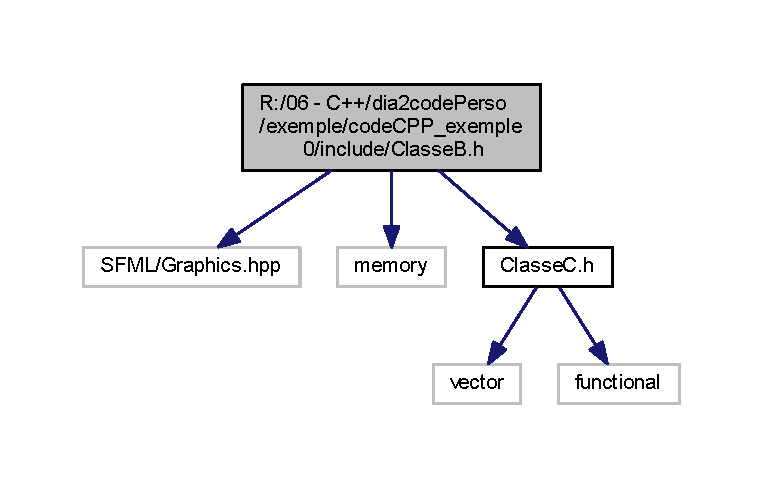
\includegraphics[width=254pt]{_classe_b_8h__incl}
\end{center}
\end{figure}
Ce graphe montre quels fichiers incluent directement ou indirectement ce fichier \+:
\nopagebreak
\begin{figure}[H]
\begin{center}
\leavevmode
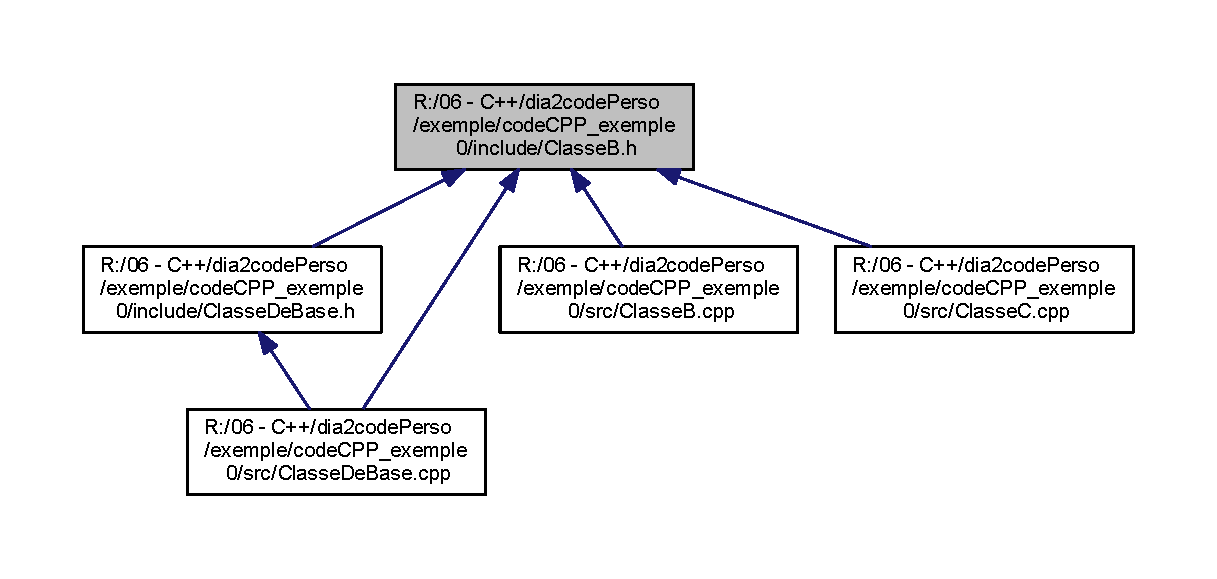
\includegraphics[width=350pt]{_classe_b_8h__dep__incl}
\end{center}
\end{figure}
\subsection*{Classes}
\begin{DoxyCompactItemize}
\item 
class {\bf Classe\+B}
\begin{DoxyCompactList}\small\item\em associé avec le type\+: \textquotesingle{}Aggregation\textquotesingle{}. Créer l\textquotesingle{}attribut dans un shared\+\_\+ptr. \end{DoxyCompactList}\end{DoxyCompactItemize}

\section{Référence du fichier R\+:/06 -\/ C++/dia2code\+Perso/exemple/code\+C\+P\+P\+\_\+exemple 0/include/\+Classe\+C.h}
\label{_classe_c_8h}\index{R\+:/06 -\/ C++/dia2code\+Perso/exemple/code\+C\+P\+P\+\_\+exemple 0/include/\+Classe\+C.\+h@{R\+:/06 -\/ C++/dia2code\+Perso/exemple/code\+C\+P\+P\+\_\+exemple 0/include/\+Classe\+C.\+h}}
{\ttfamily \#include $<$vector$>$}\\*
{\ttfamily \#include $<$functional$>$}\\*
Graphe des dépendances par inclusion de Classe\+C.\+h\+:
\nopagebreak
\begin{figure}[H]
\begin{center}
\leavevmode
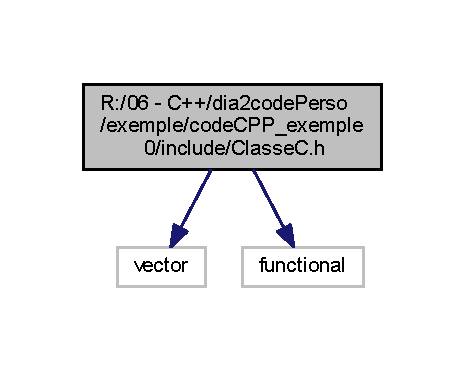
\includegraphics[width=223pt]{_classe_c_8h__incl}
\end{center}
\end{figure}
Ce graphe montre quels fichiers incluent directement ou indirectement ce fichier \+:
\nopagebreak
\begin{figure}[H]
\begin{center}
\leavevmode
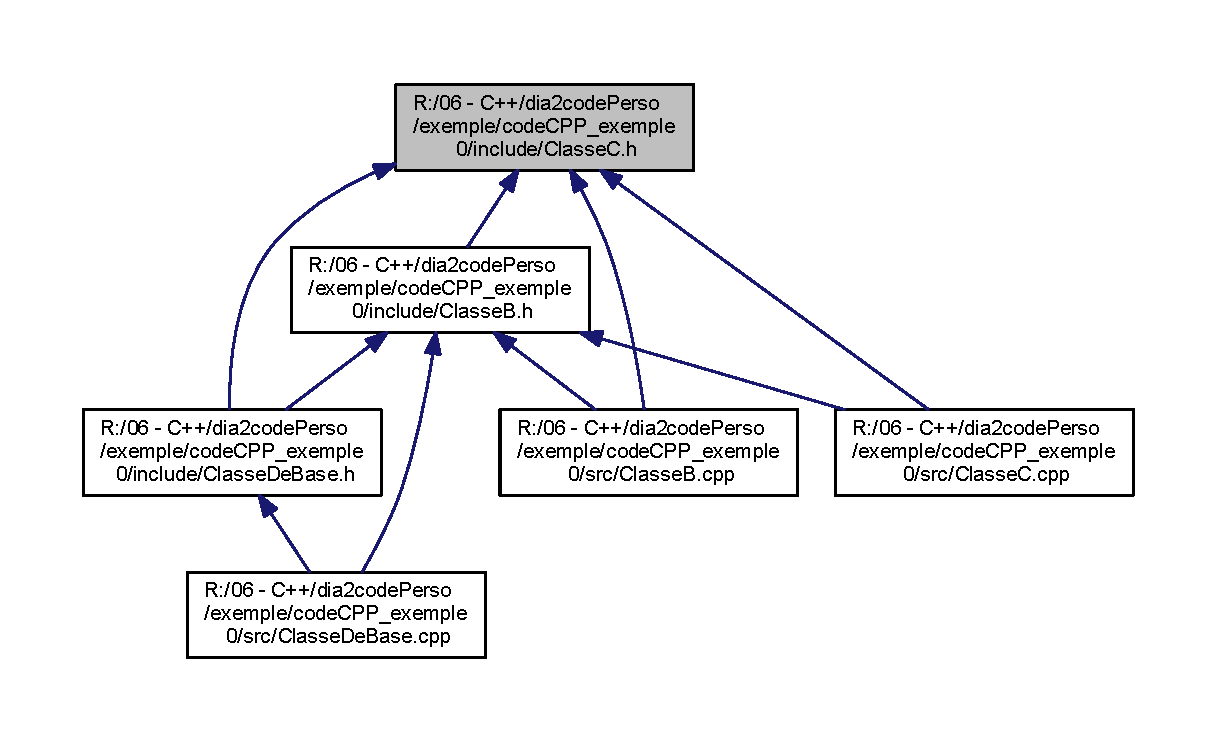
\includegraphics[width=350pt]{_classe_c_8h__dep__incl}
\end{center}
\end{figure}
\subsection*{Classes}
\begin{DoxyCompactItemize}
\item 
class {\bf Classe\+C}
\begin{DoxyCompactList}\small\item\em ici on associe 2 stereotypes \+: un using et un enum \end{DoxyCompactList}\end{DoxyCompactItemize}

\section{Référence du fichier R\+:/06 -\/ C++/dia2code\+Perso/exemple/code\+C\+P\+P\+\_\+exemple 0/include/\+Classe\+De\+Base.h}
\label{_classe_de_base_8h}\index{R\+:/06 -\/ C++/dia2code\+Perso/exemple/code\+C\+P\+P\+\_\+exemple 0/include/\+Classe\+De\+Base.\+h@{R\+:/06 -\/ C++/dia2code\+Perso/exemple/code\+C\+P\+P\+\_\+exemple 0/include/\+Classe\+De\+Base.\+h}}
{\ttfamily \#include \char`\"{}Classe\+C.\+h\char`\"{}}\\*
{\ttfamily \#include \char`\"{}Classe\+A.\+h\char`\"{}}\\*
{\ttfamily \#include $<$memory$>$}\\*
{\ttfamily \#include \char`\"{}Classe\+B.\+h\char`\"{}}\\*
Graphe des dépendances par inclusion de Classe\+De\+Base.\+h\+:
\nopagebreak
\begin{figure}[H]
\begin{center}
\leavevmode
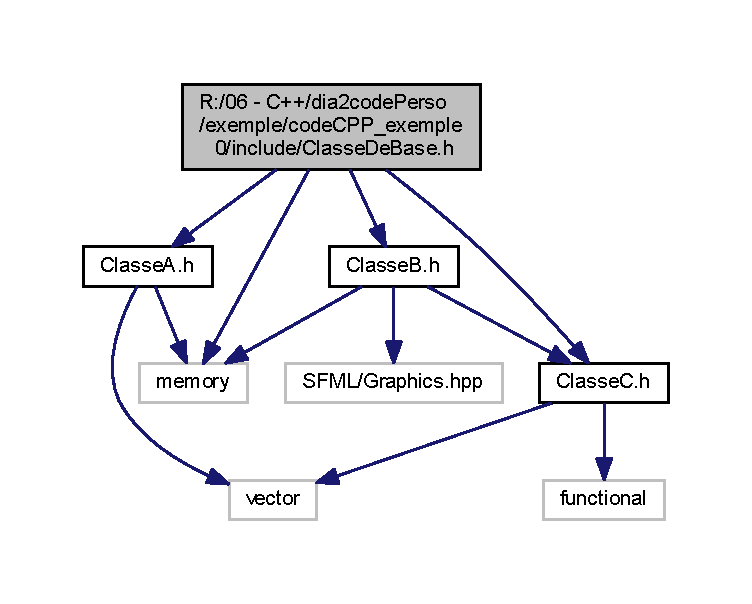
\includegraphics[width=350pt]{_classe_de_base_8h__incl}
\end{center}
\end{figure}
Ce graphe montre quels fichiers incluent directement ou indirectement ce fichier \+:\nopagebreak
\begin{figure}[H]
\begin{center}
\leavevmode
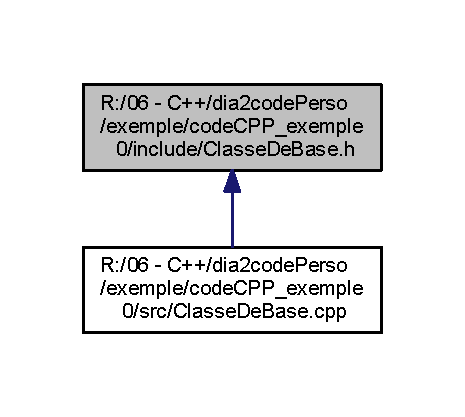
\includegraphics[width=223pt]{_classe_de_base_8h__dep__incl}
\end{center}
\end{figure}
\subsection*{Classes}
\begin{DoxyCompactItemize}
\item 
class {\bf Classe\+De\+Base}
\begin{DoxyCompactList}\small\item\em Classe qui hérite de 2 autres classes. Cela ajoutera les includes necéssaires. \end{DoxyCompactList}\end{DoxyCompactItemize}

\section{Référence du fichier R\+:/06 -\/ C++/dia2code\+Perso/exemple/code\+C\+P\+P\+\_\+exemple 0/src/\+Classe\+A.cpp}
\label{_classe_a_8cpp}\index{R\+:/06 -\/ C++/dia2code\+Perso/exemple/code\+C\+P\+P\+\_\+exemple 0/src/\+Classe\+A.\+cpp@{R\+:/06 -\/ C++/dia2code\+Perso/exemple/code\+C\+P\+P\+\_\+exemple 0/src/\+Classe\+A.\+cpp}}
{\ttfamily \#include $<$Classe\+A.\+h$>$}\\*
Graphe des dépendances par inclusion de Classe\+A.\+cpp\+:
\nopagebreak
\begin{figure}[H]
\begin{center}
\leavevmode
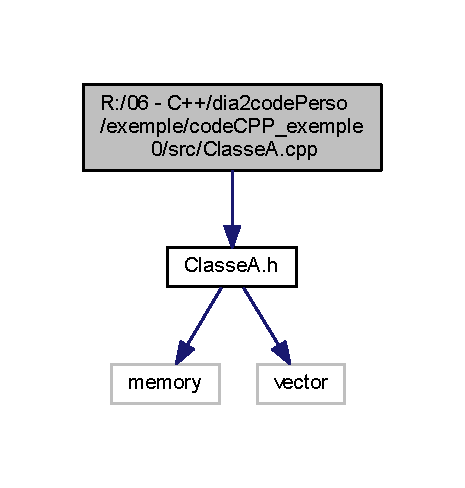
\includegraphics[width=223pt]{_classe_a_8cpp__incl}
\end{center}
\end{figure}

\section{Référence du fichier R\+:/06 -\/ C++/dia2code\+Perso/exemple/code\+C\+P\+P\+\_\+exemple 0/src/\+Classe\+B.cpp}
\label{_classe_b_8cpp}\index{R\+:/06 -\/ C++/dia2code\+Perso/exemple/code\+C\+P\+P\+\_\+exemple 0/src/\+Classe\+B.\+cpp@{R\+:/06 -\/ C++/dia2code\+Perso/exemple/code\+C\+P\+P\+\_\+exemple 0/src/\+Classe\+B.\+cpp}}
{\ttfamily \#include $<$Classe\+B.\+h$>$}\\*
{\ttfamily \#include $<$Classe\+C.\+h$>$}\\*
Graphe des dépendances par inclusion de Classe\+B.\+cpp\+:
\nopagebreak
\begin{figure}[H]
\begin{center}
\leavevmode
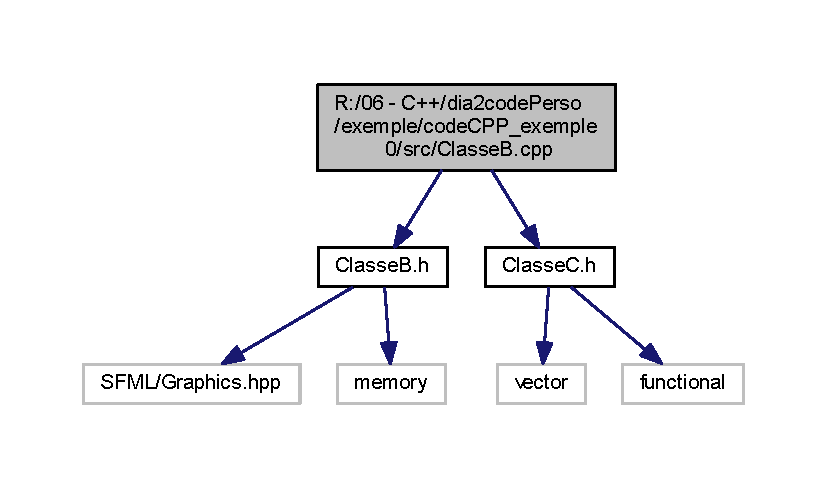
\includegraphics[width=350pt]{_classe_b_8cpp__incl}
\end{center}
\end{figure}

\section{Référence du fichier R\+:/06 -\/ C++/dia2code\+Perso/exemple/code\+C\+P\+P\+\_\+exemple 0/src/\+Classe\+C.cpp}
\label{_classe_c_8cpp}\index{R\+:/06 -\/ C++/dia2code\+Perso/exemple/code\+C\+P\+P\+\_\+exemple 0/src/\+Classe\+C.\+cpp@{R\+:/06 -\/ C++/dia2code\+Perso/exemple/code\+C\+P\+P\+\_\+exemple 0/src/\+Classe\+C.\+cpp}}
{\ttfamily \#include $<$Classe\+C.\+h$>$}\\*
{\ttfamily \#include $<$Classe\+A.\+h$>$}\\*
Graphe des dépendances par inclusion de Classe\+C.\+cpp\+:
\nopagebreak
\begin{figure}[H]
\begin{center}
\leavevmode
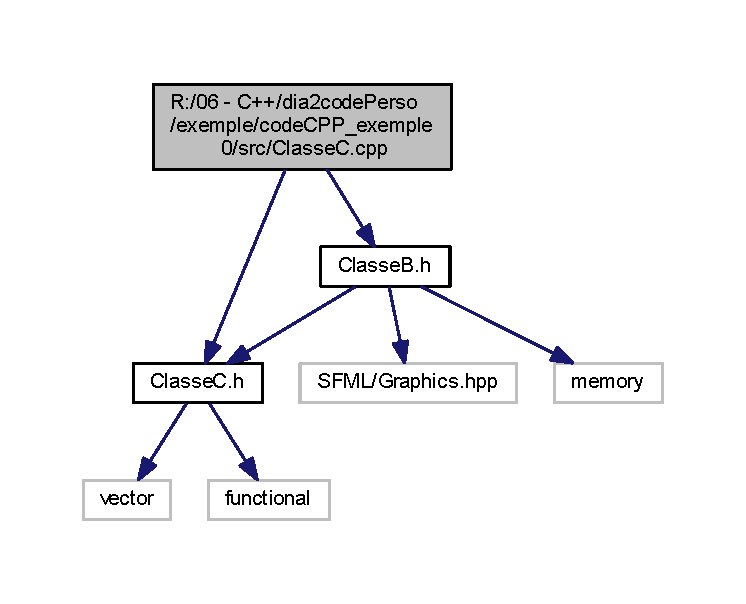
\includegraphics[width=268pt]{_classe_c_8cpp__incl}
\end{center}
\end{figure}

\section{Référence du fichier R\+:/06 -\/ C++/dia2code\+Perso/exemple/code\+C\+P\+P\+\_\+exemple 0/src/\+Classe\+De\+Base.cpp}
\label{_classe_de_base_8cpp}\index{R\+:/06 -\/ C++/dia2code\+Perso/exemple/code\+C\+P\+P\+\_\+exemple 0/src/\+Classe\+De\+Base.\+cpp@{R\+:/06 -\/ C++/dia2code\+Perso/exemple/code\+C\+P\+P\+\_\+exemple 0/src/\+Classe\+De\+Base.\+cpp}}
{\ttfamily \#include $<$Classe\+De\+Base.\+h$>$}\\*
{\ttfamily \#include $<$Classe\+B.\+h$>$}\\*
Graphe des dépendances par inclusion de Classe\+De\+Base.\+cpp\+:\nopagebreak
\begin{figure}[H]
\begin{center}
\leavevmode
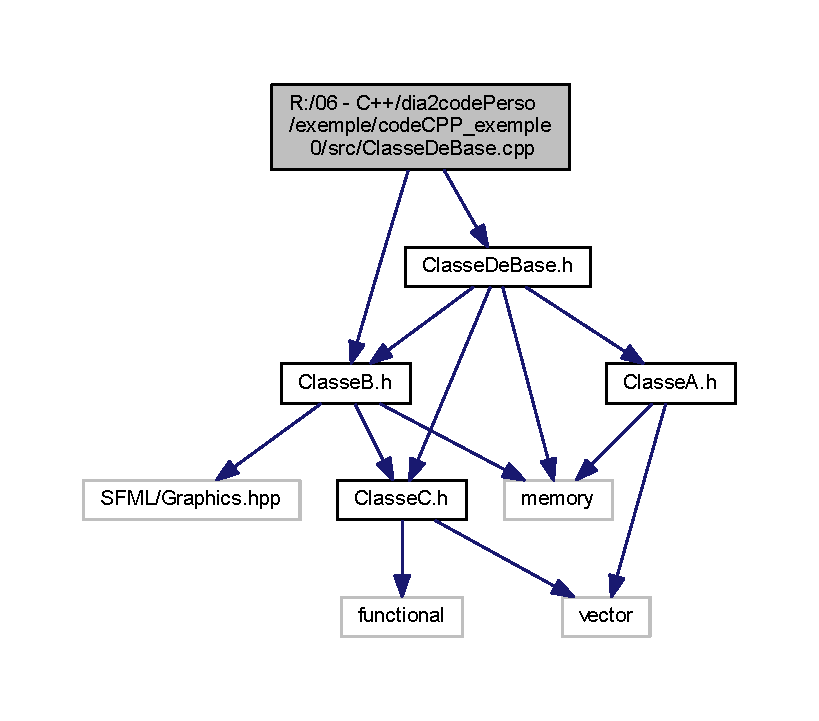
\includegraphics[width=350pt]{_classe_de_base_8cpp__incl}
\end{center}
\end{figure}

%--- End generated contents ---

% Index
\backmatter
\newpage
\phantomsection
\clearemptydoublepage
\addcontentsline{toc}{chapter}{Index}
\printindex

\end{document}
